\documentclass[11pt,a4paper]{article}
\usepackage[margin=2.3cm]{geometry}
\usepackage{graphicx,booktabs,amsmath,amssymb,hyperref,textcomp}
\usepackage[T1]{fontenc}
\usepackage{lmodern}
\hypersetup{colorlinks,linkcolor=black,citecolor=black,urlcolor=blue!50!black}
\title{A six-equation two-pressure code against the ECCSEL CO$_2$ depressurization tests:\\ the nucleation onset, the transfer rate, and what an HRM-type source shows}
\author{M.\ Day\thanks{Prepared with an AI assistant from the runs recorded on branch \texttt{co2-eos} of CAMR (tag \texttt{onset-2026-09-23}); every number is from a recorded run.}}
\date{23 September 2026 --- draft for discussion, revised}
\begin{document}
\maketitle

\section*{Purpose}
Log, Hammer, Deng, Austegard, Hafner and Munkejord (\emph{Int.\ J.\ Multiphase Flow} 170 (2024) 104624) published seven full-bore depressurizations of dense liquid-like CO$_2$ in the ECCSEL pipe, with pressure traces at 100\,kHz near the open end, and compared them with a homogeneous equilibrium model (HEM) and a $pT$-relaxed homogeneous relaxation model (HRM$^*$) whose single relaxation time $\theta$ was fitted per test. This note runs three of those tests with CAMR, a six-equation Pelanti--Shyue two-pressure code, and reports three things: what the code's closure gets right and wrong against the measurements; that replacing the code's fixed nucleation margin by the classical-nucleation-theory onset reproduces the warm test's first level with nothing fitted; and what happens when the paper's source law is placed inside the two-pressure model. It is a basis for discussion, not a validation claim: the runs are one-dimensional, adiabatic and frictionless over the last 3--4\,m of the pipe and the first 10\,ms, and the transfer rate behind the onset remains the open closure.

\section{The comparison}
\paragraph{Tests.} Test 19 (124.7\,bar, 10.2\,\textdegree C; the paper's $\theta$ = 2.5\,ms), Test 23 (121.9\,bar, 31.5\,\textdegree C; $\theta$ = 0.55\,ms; held out until the onset law was fixed) and Test 24 (115.6\,bar, 35.8\,\textdegree C; $\theta$ = 0.14\,ms). Sensors PT201--PT206 at 0.08, 0.18, 0.28, 0.484, 0.8 and 1.599\,m from the open end; uncertainty about 0.6\,bar.

\paragraph{CAMR.} Six-equation model with instantaneous mechanical relaxation, a coupled pressure--temperature--Gibbs relaxation operator (X3) whose mass transfer uses a statistical-rate-theory (SRT) rate with an interfacial-area prefactor $\Sigma \propto (\alpha_2+\delta)\alpha_1/D$ ($\delta = 0.01$, morphology length $D$, default 0.1\,m), second-order wave-propagation hydrodynamics, 6.25\,mm cells (the paper: 6.17\,mm). A single-phase liquid below saturation acquires vapour through a \emph{nucleator}: a smooth window in pressure that opens at $(1 - m)P_{\mathrm{sat}}(T)$ and seeds vapour to a volume fraction of 0.04; the committed fraction is solved implicitly in the window. Until this work the margin was a constant, $m = 0.1$. It is now the homogeneous-nucleation onset at the liquid's temperature,
\[ J = N_\ell\sqrt{2\sigma/\pi m_1}\;\exp\!\big[-16\pi\sigma^3/(3k_BT\,\Delta P^2)\big] = 10^{12}\ \mathrm{m^{-3}s^{-1}},\qquad \Delta P = (P_{\mathrm{sat}} - P)(1 - \rho_v/\rho_\ell), \]
with the paper's Appendix~A threshold and $\sigma(T) = 0.07863\,(1 - T/T_c)^{1.254}$\,N/m (Mulero et al.\ 2012), capped at the former constant: $m(T) = \min(m_{\mathrm{CNT}}, 0.1)$. Nothing is fitted; the cap is the heterogeneous (wall) floor the cold data require. The two runs of each test below are ``fixed window'' (the former default) and ``CNT onset'' (the present one). The outlet is a characteristic face with an outflow fan; the far end of the truncated domain is a wall the wave never returns from. EOS: GERG-2008 for every run shown; Peng--Robinson for the parameter scans of Fig.~\ref{fd}.

\paragraph{The HRM-source probe.} A switch replaced the nucleator by the paper's source, $\Gamma = \rho\,(x_{g,\mathrm{sat}} - x_g)/\theta$, active in every cell whose liquid is below $P_{\mathrm{sat}}(T)$, with $x_{g,\mathrm{sat}}$ the equilibrium quality at the cell's $(\rho, e)$ on the EOS's own dome, the SRT transfer switched off, and the instantaneous mechanical and thermal relaxation kept --- the $pT$-relaxed assumption of HRM$^*$ inside the two-pressure model. A probe of one question (Fig.~\ref{f19}, PR), not a proposed closure; it is not in the code.

\section{Results}
\begin{figure}[htbp]\centering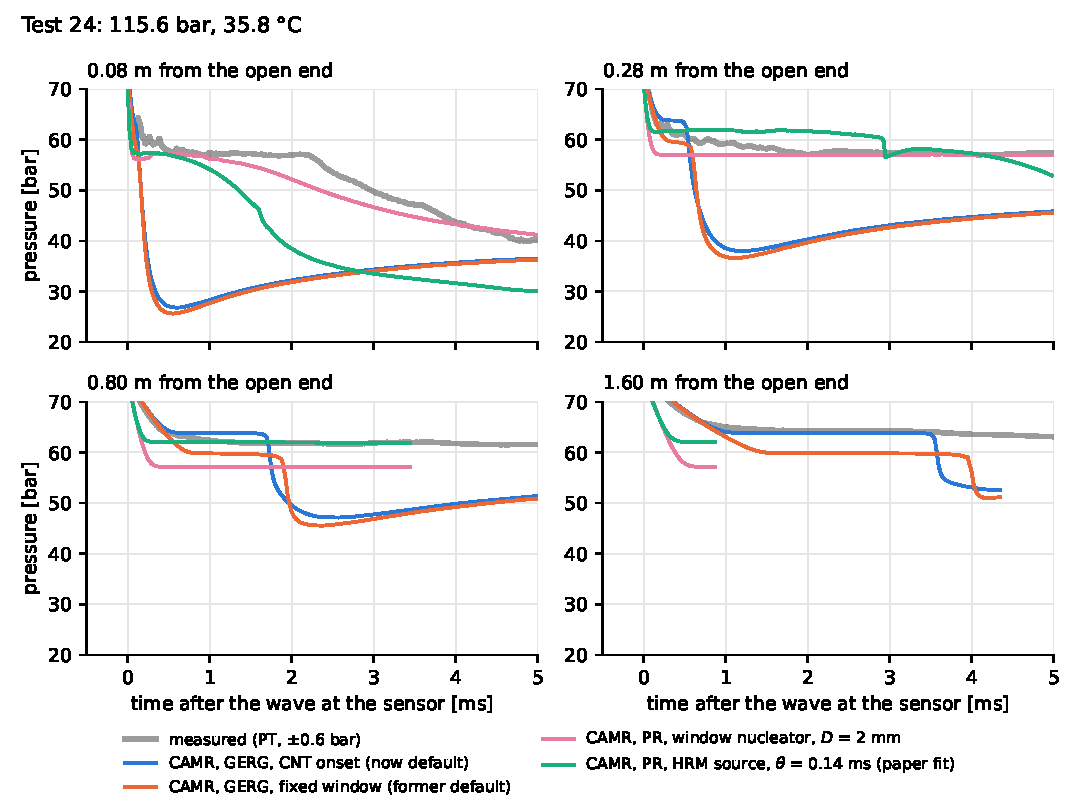
\includegraphics[width=\textwidth]{fig_test24.pdf}
\caption{Test 24 (warm). Every trace is shifted so that its 40\,bar drop at the sensor is $t = 0$ (the rupture disk opens over milliseconds; the code opens instantly), so absolute times are not comparable while levels and times after the wave are. The CNT onset lifts the first level from $0.92$ to $0.98\,P_{\mathrm{sat}}$; what follows it, the fall to 48\,bar at 2\,ms, is the transfer rate and is unchanged. The pink trace is the fixed window with the SRT morphology length reduced from 0.1\,m to 2\,mm.}\label{f24}\end{figure}
\begin{figure}[htbp]\centering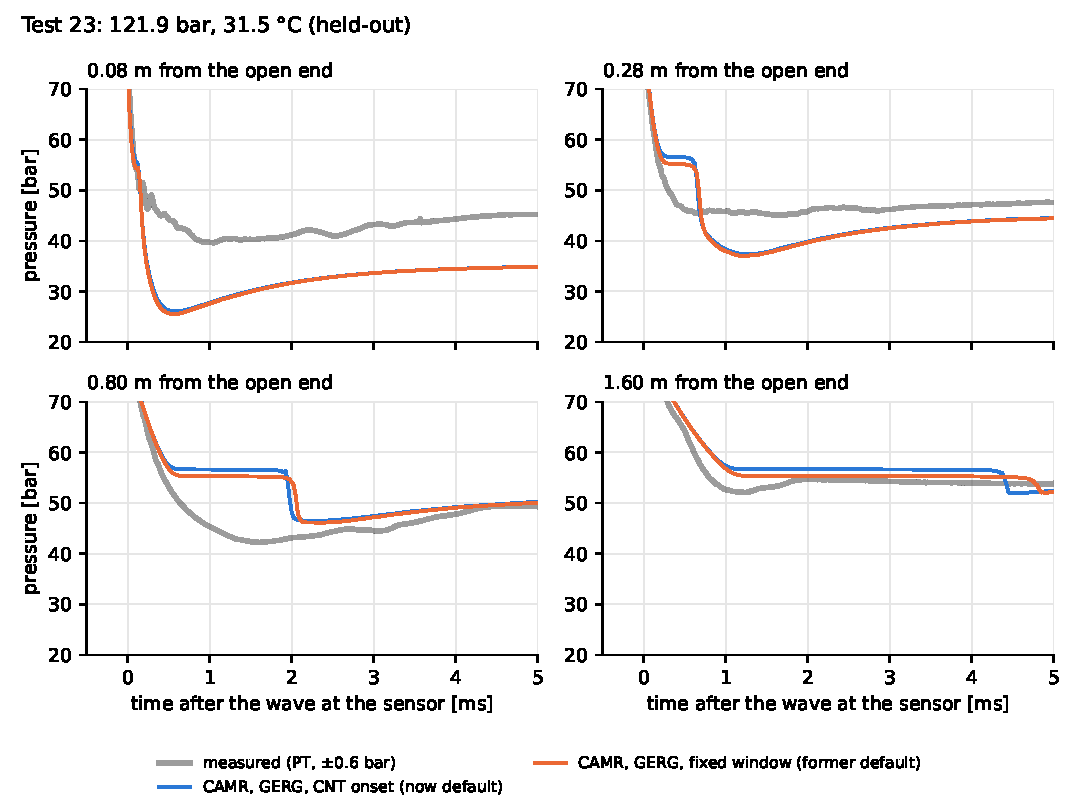
\includegraphics[width=\textwidth]{fig_test23.pdf}
\caption{Test 23 (31.5\,\textdegree C, held out). The measurement has no plateau near saturation: it falls 13\,bar past the onset and recovers 6\,bar. Both onset laws put the first level where they say (56.7 and 55.4\,bar at 0.8\,m); neither follows the dip, which the transfer rate governs. The CNT run leaves its plateau a millisecond earlier.}\label{f23}\end{figure}
\begin{figure}[htbp]\centering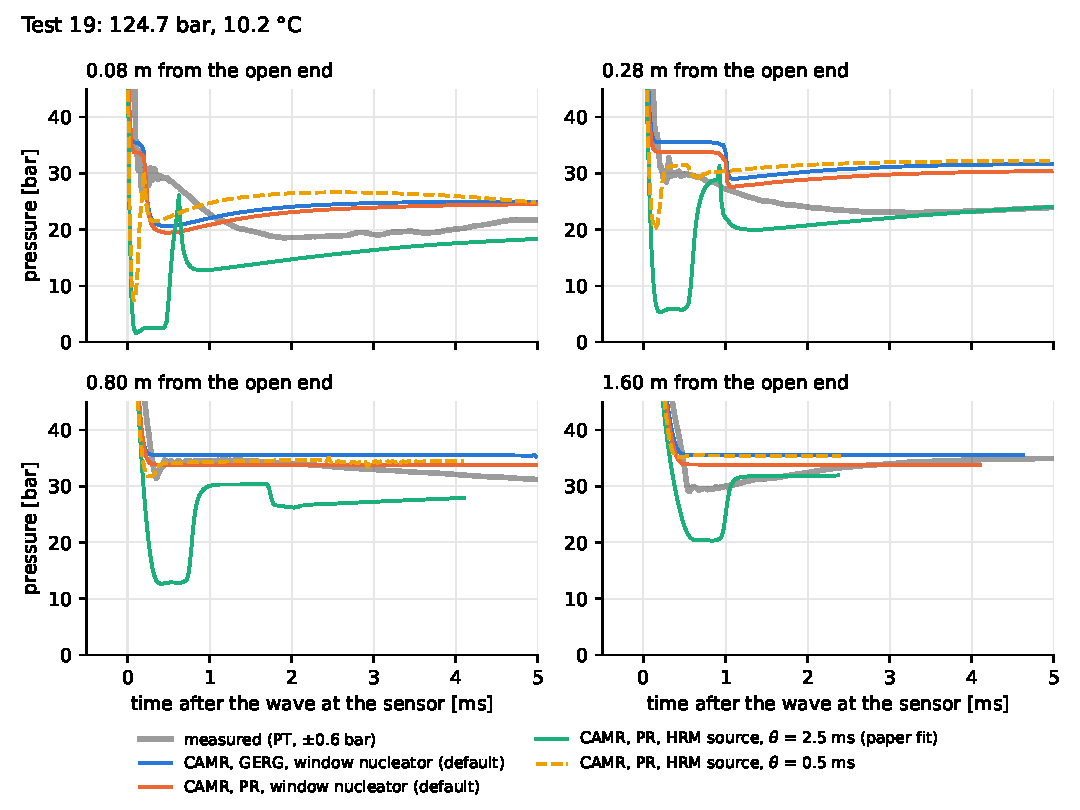
\includegraphics[width=\textwidth]{fig_test19.pdf}
\caption{Test 19 (cold). The CNT-onset run is identical to the fixed window (the cap binds: the homogeneous limit would be a 63\,\% undershoot at 276\,K against a measured 9\,\%). The green traces are the HRM-source probe (PR) at the paper's $\theta$ and at 0.5\,ms: the undershoot and recovery appear at the measured times after the wave.}\label{f19}\end{figure}
\begin{figure}[htbp]\centering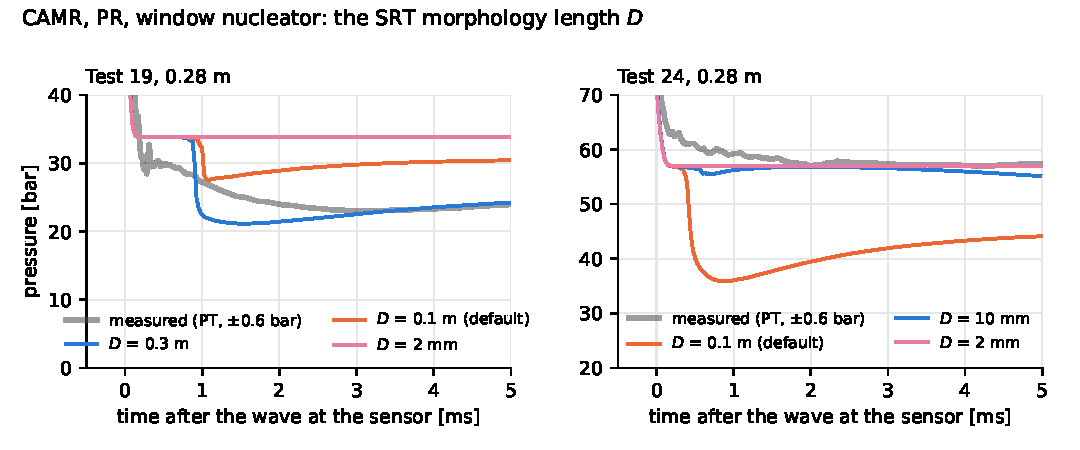
\includegraphics[width=\textwidth]{fig_dscan.pdf}
\caption{The morphology length $D$ of the SRT rate, fixed window, PR, at the 0.28\,m sensor: the cold test wants $D \approx 0.2$\,m, the warm one $D \lesssim 2$\,mm.}\label{fd}\end{figure}

\begin{table}[htbp]\centering\scriptsize\setlength{\tabcolsep}{2.5pt}
\caption{Numbers behind the figures (GERG unless marked PR). ``Level'' is the first plateau after the fast drop; for Test 23 the measured value is the bottom of the dip, not a plateau. HRM$^*$ rows are the paper's statements about its own model; its traces are not reproduced here.}
\begin{tabular}{llccp{2.7cm}p{2.1cm}}\toprule
& & wave speed & level, 0.8\,m & dip $\to$ max, 0.8\,m & 0.08\,m at $+5$\,ms\\
& & 0.8$\to$3.2\,m [m/s] & [bar] & [bar] & [bar]\\\midrule
Test 24 & measured & 370 & 63.8 & flat & 40.4\\
& HRM$^*$, $\theta$ = 0.14\,ms & --- & --- & no plateau; drop too slow & overestimates\\
& CAMR, fixed window & 366 & 60.0 & flat & 36.9 at 10\,ms (meas.\ 37.2)\\
& CAMR, CNT onset & 366 & 64.0 & flat & 36.5\\
& CAMR PR, fixed window, $D$ = 2\,mm & --- & 57.1 & flat & 41.2\\
& CAMR PR, HRM source, 0.14\,ms & --- & 62.0 & flat & 30.0\\\midrule
Test 23 & measured & 441 & 42.9 (dip) & $53 \to 43 \to 49$ & 45.2\\
& CAMR, fixed window & 419 & 55.4 & $55.3 \to 47$, no recovery & 34.9\\
& CAMR, CNT onset & 419 & 56.7 & $56.6 \to 47$, no recovery & 34.9\\\midrule
Test 19 & measured & 585 & 34.2 & $32.5 \to 34.6$ & 21.8\\
& HRM$^*$, $\theta$ = 2.5\,ms & --- & --- & captured (fitted); recovery ``more abrupt'' than measured & underestimates\\
& CAMR, fixed window & 592 & 35.6 & flat & 25\\
& CAMR, CNT onset & 592 & 35.6 (identical) & flat & 25\\
& CAMR PR, HRM source, 2.5\,ms & --- & --- & $12.7 \to 30.3$ & 18.4\\
& CAMR PR, HRM source, 0.5\,ms & --- & --- & $31.8 \to 34.8$ & 24.8\\\bottomrule
\end{tabular}\end{table}

\paragraph{What the two-pressure model gets right without tuning.} The head of the depressurization wave travels at the measured speed (within 1.2\,\% at both ends; 5\,\% low on Test 23), and with the CNT onset the first level after the fast drop is within 0.2\,bar of the measurement warm (64.0 vs.\ 63.8\,bar) and 1.4\,bar cold (35.6 vs.\ 34.2). The warm number was predicted before the run (64.0 $\pm$ 0.5) from the law alone. The choked outlet pressure of the warm test at 10\,ms is reproduced (36.5 vs.\ 37.2\,bar).

\paragraph{What the onset law does and does not do.} Near the critical point $\sigma \to 0$ and the homogeneous onset is at saturation ($m$ = 0.023 at 298.5\,K), which is what Test 24 shows. Far from it the homogeneous limit is unreachable in a pipe (63\,\% at 276\,K) and the cap governs; the cold onset is therefore \emph{not predicted} by this law, only left at the former constant, which the data happen to put near 9--10\,\%. A wall-nucleation law would replace the cap; that needs a site density and a contact angle the data do not supply.

\paragraph{What the transfer rate does not do.} Behind the first level the code's SRT rate at the default morphology length is far too slow warm (Fig.~\ref{f24}: 48\,bar at 2\,ms against 62) and somewhat too fast cold; the two tests bracket $D$ at 0.2\,m and $\lesssim 2$\,mm (Fig.~\ref{fd}), a range of 100 against the paper's 18:1 in $\theta$. Test 23 is the sharpest statement of the same deficiency: at 31.5\,\textdegree C the onset is right and the measured pressure still falls 13\,bar below it and recovers 6, while the code holds its plateau (Fig.~\ref{f23}). There is no undershoot-and-recovery in any CAMR run, because the window pins the liquid at the onset and nothing keeps producing vapour once the pressure rises.

\paragraph{What the HRM source inside the two-pressure model does.} With the paper's source law the code produces the undershoot and the recovery (Fig.~\ref{f19}), at the measured time after the wave (0.40 and 0.82\,ms against 0.33 and 0.79\,ms at 0.8 and 1.6\,m). So the two-pressure structure and the trace-phase treatment are not the obstacle; the feature needs a source that starts at the saturation line, is at full strength with no vapour present, and keeps producing while the pressure recovers. A transported interfacial-area density was also tried, coupled into the SRT rate, and refuted: it only rescaled the transfer and gave no recovery.

\paragraph{Two things we would like to discuss.}
\begin{enumerate}
\item At the paper's fitted $\theta$ = 2.5\,ms our dip is far deeper than the measurement (12.7\,bar at 0.8\,m against 32.5); $\theta$ = 0.5\,ms reproduces that sensor within 1\,bar but is 5--8\,bar high nearer the outlet. We do not know how much of the difference at equal $\theta$ is the hydrodynamics (second-order wave propagation against first-order HLLC), the definition of $x_{g,\mathrm{sat}}$ (ours: the equilibrium quality at the cell's $(\rho,e)$), or the outlet condition (our vent chokes on the equilibrium path; the paper's minimum BBC is built not to restrain the non-equilibrium). The authors' HRM$^*$ traces at 0.8 and 1.6\,m for Tests 19 and 23 would separate these.
\item The onset near the critical point is homogeneous CNT with no free constant, and the cold onset is a wall property; between them Test 23 shows the transfer, not the onset, setting the dip. Does the authors' nucleation-onset analysis (their Figs.\ 19--20) support a local growth law --- conduction-limited bubble growth in the liquid's superheat, say --- that could carry the 100:1 range in $D$ without a per-test constant? That is the closure we would build next.
\end{enumerate}

\paragraph{Caveats.} One-dimensional, no wall friction or heat transfer, no disk-opening model, adiabatic; the last 3--4\,m of the pipe only, so nothing here speaks to the plateau after 10\,ms. The measured traces are the authors' public dataset (doi 10.5281/zenodo.7669536, CC BY 4.0).
\end{document}
